\section{Krisescenario og svikt i dagens beredskap}
\label{sec:scenariet}

\subsection{Det akutte forurensningsscenariet}
Norsk drikkevannsforsyning er basert på sårbare overflatekilder. Scenarioet tar utgangspunkt i en norsk by med \num{50000} til \num{100000} innbyggere som rammes av et intensivt flomforløp etter ekstremnedbør. Flomvannet overbelaster fellesavløpsnettet, hvorpå tilbakeslag og oversvømte pumpestasjoner medfører massivt urenset kloakkoverløp i byens primære råvannskilde og sentrale høydebasseng.

Vannet kontamineres akutt med patogene mikroorganismer, primært \textit{Campylobacter jejuni}, enteropatogene \textit{Escherichia coli} og norovirus. Før rutineanalyser rekker å stanse distribusjonen, har smittestoffene spredt seg i rørnettet. Kommuneoverlegen beordrer umiddelbar stenging av nettet for konsum ledsaget av kokevarsel. Byen står overfor en akutt helse- og forsyningskrise.

\subsection{Hvorfor etablert beredskap svikter}
Når ledningsnettet settes ut av spill, kollapser tradisjonelle krisetiltak i løpet av timer:
\begin{enumerate}[leftmargin=1.5em, itemsep=0.2em]
    \item \textbf{Flaskevann-kollaps:} Dagligvarehandelen opererer med slanke «just-in-time»-lagre, og butikkhyller tømmes innen tre timer. Palltransport av flaskevann er logistisk ineffektivt grunnet emballasjevekt og dødvolum; å dekke dagsbehovet til \num{75000} innbyggere krever over 20 semitrailere daglig, med uoverkommelige trafikkpropper som resultat.
    \item \textbf{Institusjonell lammelse:} Kokevarsel fungerer for friske husholdninger, men lammer helseinstitusjoner. Akuttsykehus, sykehjem og dialyseenheter krever titusenvis av liter sterilt vann daglig til pasientbehandling, sårstell, dialyse, hygiene og matproduksjon. Helseforetakene mangler kjelekapasitet og personell til storskala koking og nedkjøling.
    \item \textbf{Forurenset kommunalt materiell:} Brann- og spylebiler kan ikke benyttes til drikkevann. Tanker og slanger inneholder rust, etablert biofilm samt giftige rester av kjemikalier og \textsc{pfas}-holdig slukkeskum som ikke lar seg dekontaminere i felten.
    \item \textbf{Mangel på bulkbeholdere:} Kommuner disponerer knapt sertifiserte næringsmiddeltanker for bulktransport. Innleie tar dager, mens behovet for rent vann er akutt.
\end{enumerate}

Dermed oppstår et livstruende kapasitetsgap: Byen trenger storskala distribusjon av sterilt drikkevann, men mangler mobile, godkjente beholdere. Som vist i figur~\ref{fig:kart} etablerer Prosjekt Meierikjeden en mobil forsyningskjede over vei som bypasser det forurensede rørnettet.

\begin{figure}[htbp]
    \centering
    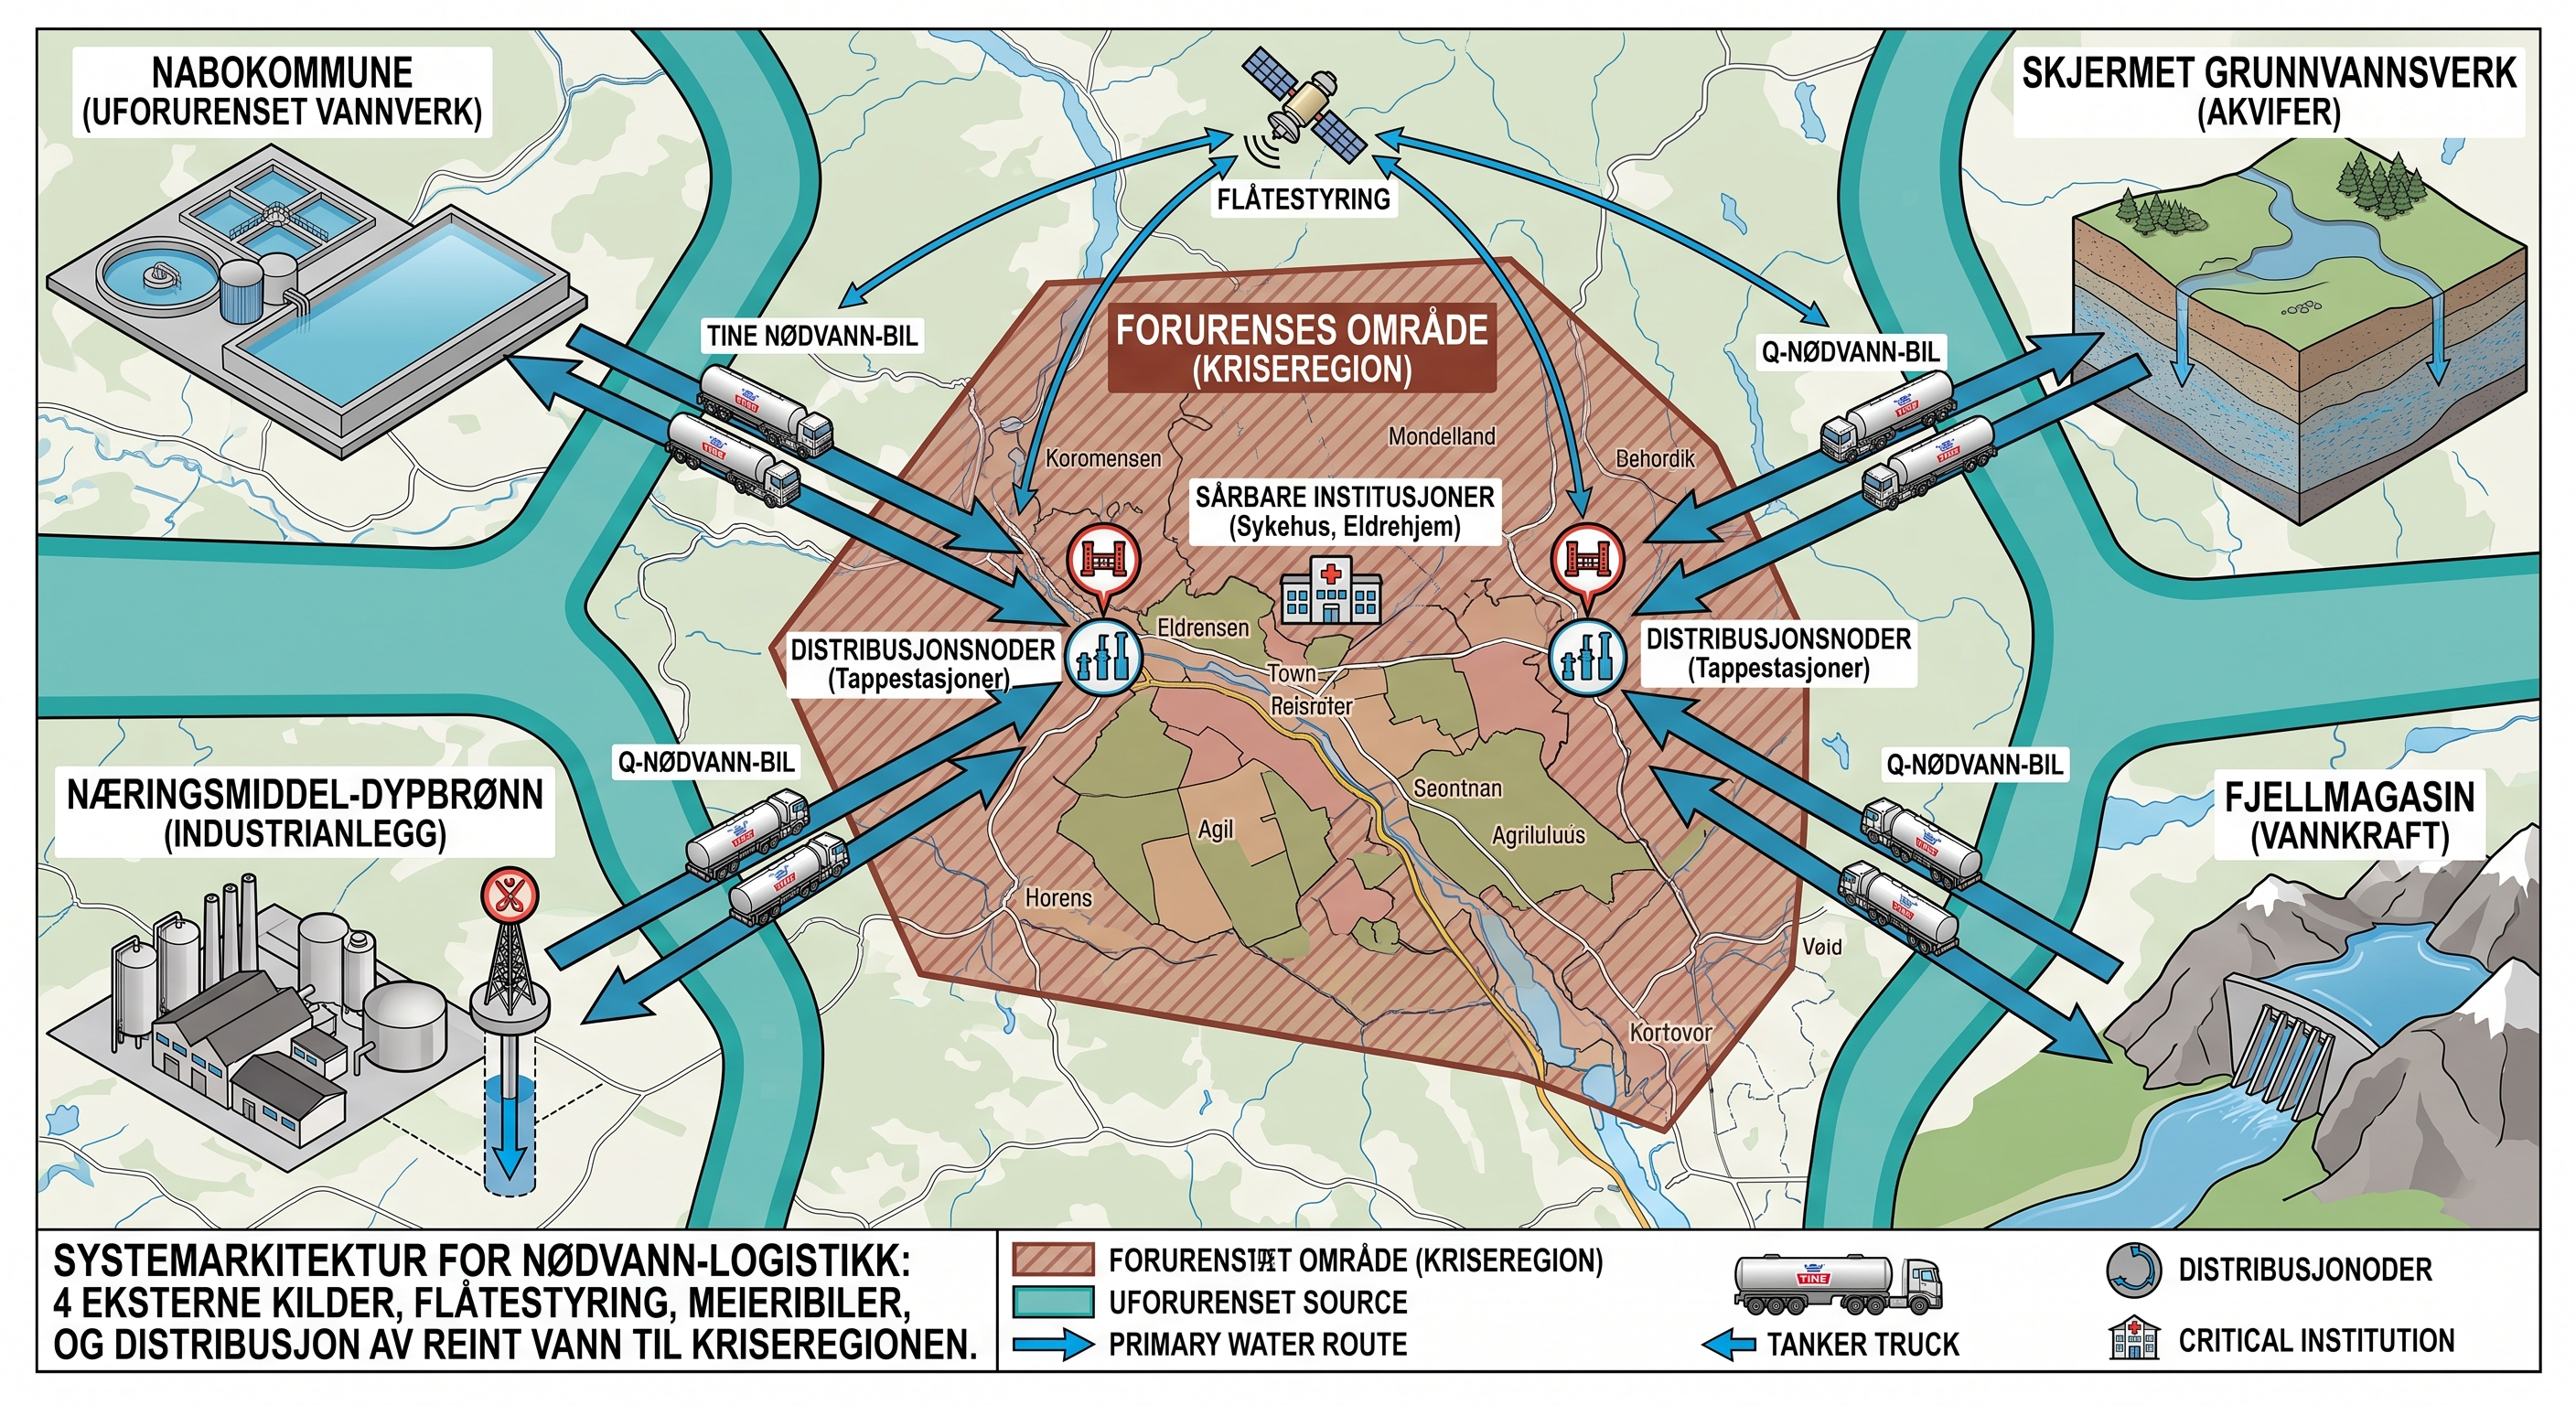
\includegraphics[width=0.95\textwidth]{Figures/Kart_over_forskyningskjede.jpg}
    \caption{Systemarkitektur for Prosjekt Meierikjeden: Mobilisering av meieriflåten etablerer en «virtuell rørledning» over vei fra fire uavhengige reservekilder, med to-spors forsyning til sykehus (Linje A) og sivile utdelingspunkter (Linje B).}
    \label{fig:kart}
\end{figure}
